\documentclass{article} % Класс печатного документа

% для поддержки русского языка
\usepackage[T2A]{fontenc} % поддержка специальных русских символов
\usepackage[utf8]{inputenc} % Кодировка исходного текста - utf8
\usepackage[english,russian]{babel} % Поддержка языка - русского с английским
\usepackage{indentfirst} % Отступ в первом абзаце

\usepackage{hyperref} % Для вставки гиперссылок
% \usepackage{listings} % Для вставки кусков кода
\usepackage{graphicx} % Вставка изображений
\usepackage{subfig} % Изображения друг напротив друга
\usepackage{float} % Для точного позиционирования картинок
\usepackage[justification=centering]{caption} % Для центрирования подписей

% Default fixed font does not support bold face
\DeclareFixedFont{\ttb}{T1}{txtt}{bx}{n}{12} % for bold
\DeclareFixedFont{\ttm}{T1}{txtt}{m}{n}{12}  % for normal

% Custom colors
\usepackage{color}
\definecolor{deepblue}{rgb}{0,0,0.5}
\definecolor{deepred}{rgb}{0.6,0,0}
\definecolor{deepgreen}{rgb}{0,0.5,0}

\usepackage{listings}

% Python style for highlighting
\newcommand\pythonstyle{\lstset{
    language=Python,
    basicstyle=\ttm,
    otherkeywords={self},             % Add keywords here
    keywordstyle=\color{deepblue},
    emph={MyClass,__init__},          % Custom highlighting
    emphstyle=\color{deepred},    % Custom highlighting style
    stringstyle=\color{deepgreen},
    frame=tb,                         % Any extra options here
    showstringspaces=false,           % 
    basicstyle=\small,                % уменьшить размер шрифта
    columns=flexible                  % чтобы при копировании не было пробелов везде
}}


% Python environment
\lstnewenvironment{python}[1][]
{
\pythonstyle
\lstset{#1}
}
{}

% Python for external files
\newcommand\pythonexternal[2][]{{
\pythonstyle
\lstinputlisting[#1]{#2}}}

% Python for inline
\newcommand\pythoninline[1]{{\pythonstyle\lstinline!#1!}}

\makeatletter
\def\lst@outputspace{{\ifx\lst@bkgcolor\empty\color{white}\else\lst@bkgcolor\fi\lst@visiblespace}}
\makeatother
 % для красивого оформления python кода

% путь к папке с изображениями
\graphicspath{{./figs/}}

\title{Отчёт 10\\
Мультиклассовая классификация\\
с помощью методов Random Forest (RF)\\
и Gradient Boosting (GB)} % заголовок документа
\author{Свичкарев А.\,В.} % Автор документа
\date{\today} % Текущая дата

\begin{document} % Конец преамбулы, начало текста

\maketitle % Печатает заголовок, список авторов и дату

\section{Цель}
Изучить способы решения задач мультиклассовой классификации
данных с применением методов Random Forest (RF) и Gradient Boosting (GB).

\section{Задание №1}
Написать программу построения модели классификации данных
glass.data.csv методом случайного из файла
леса деревьев решений (Random Forest) и
визуализации деревьев решений.
Построить и визуализировать частные модели деревьев,
на основе которых построить модель предсказания классов данных.
Привести значение минимальной ошибки (Missclassification Error),
график зависимости ошибок (Missclassification Error Rate)
от числа деревьев в ансамбле и матрицу ошибок (Confusion Matrix).
Оценить точность классификации при различных значениях
параметра max\_depth (1,3,5).
\bigskip

Реализация на основе кода программы из Приложения.

\clearpage
Примеры частных моделей деревьев:
\begin{figure}[H]
	\centering
	\subfloat[Первое дерево]{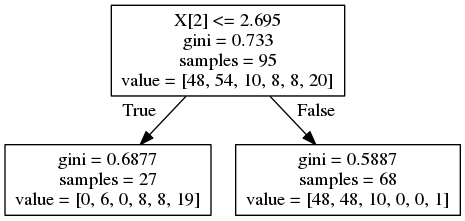
\includegraphics[width=0.5\textwidth]{tree1Ex1.png}}
	\hfill
	\subfloat[Второе дерево]{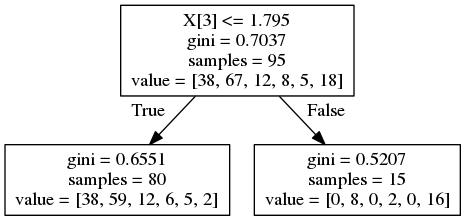
\includegraphics[width=0.5\textwidth]{tree2Ex1.png}}
    \caption{Графические построения деревьев глубины 1}
\end{figure}
\bigskip

Значения минимальной ошибки (Missclassification Error Rate)
от числа деревьев в ансамбле и матрица ошибок (Confusion Matrix).
при различных величинах глубины деревьев:
\lstinputlisting{./ex1_out.txt}

\begin{figure}[H]
    \centering
    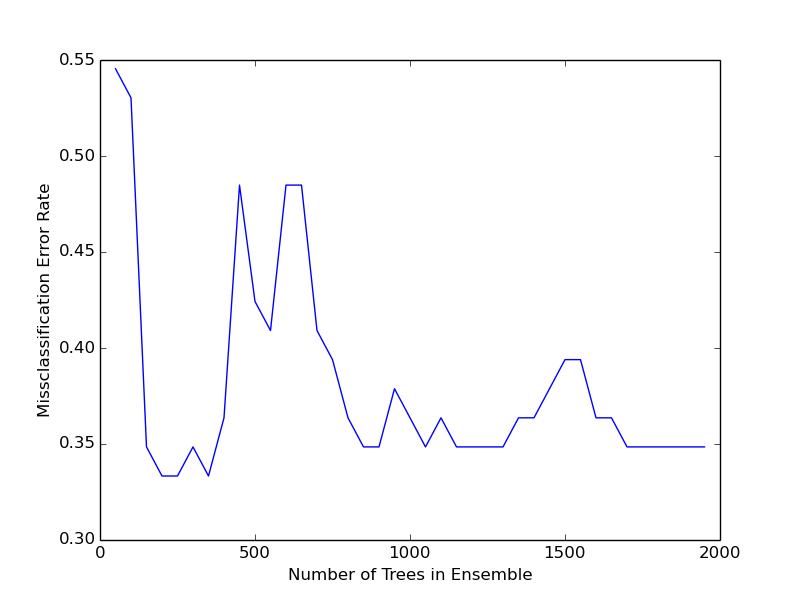
\includegraphics[width=\textwidth]{mer1depth}
    \caption{График зависимости ошибок от числа деревьев в ансамбле (Missclassification Error Rate}
\end{figure}

\begin{figure}[H]
    \centering
    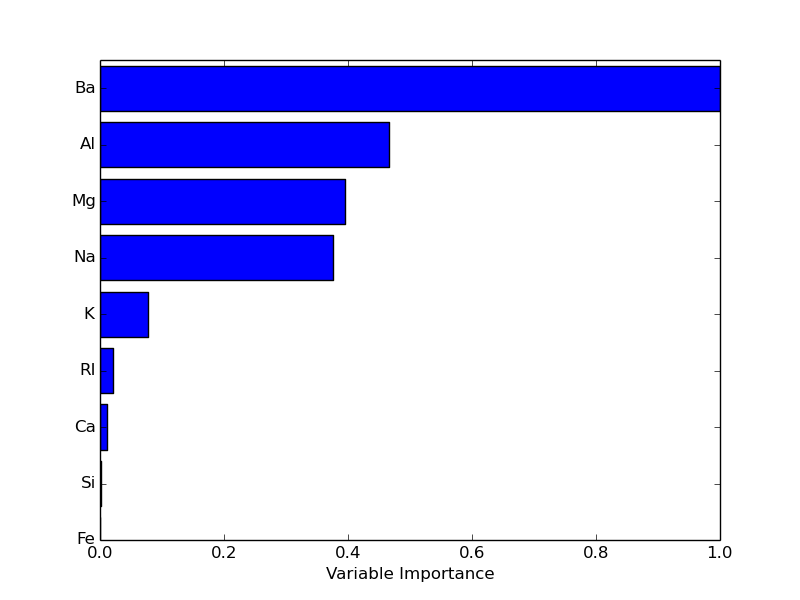
\includegraphics[width=\textwidth]{varImp1depth.png}
    \caption{Относительная важность различных атрибутов (Variable Importance)}
\end{figure}

\clearpage
\section{Задание №2}
Выполнить классификацию данных из файла glass.data.csv
методом методом Gradient Boosting и визуализировать деревья решений.
Привести результаты классификации данных.
Оценить точность классификации при различных значениях параметра
max\_depth (1,3,5).

Сравнить эффективность двух методов (RF и GB).
\bigskip

Реализация на основе кода программы из Приложения.

\clearpage
Примеры частных моделей деревьев:

\begin{figure}[H]
	\centering
	\subfloat[Первое дерево]{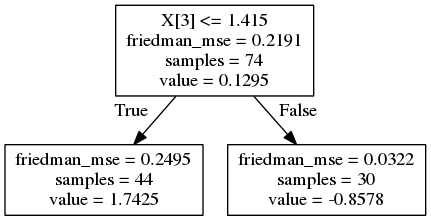
\includegraphics[width=0.5\textwidth]{tree1Ex2.png}}
	\hfill
	\subfloat[Второе дерево]{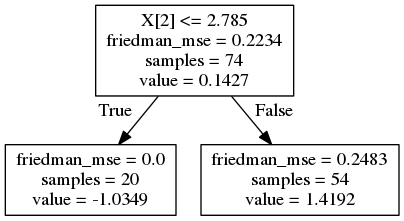
\includegraphics[width=0.5\textwidth]{tree2Ex2.png}}
    \caption{Графические построения деревьев глубины 1}
\end{figure}
\bigskip

Значение минимального среднего квадрата ошибки Minimum MSE
при различных параметрах (закодированы в названиях файлов):

% \begin{figure}[H]
% 	\centering
% 	\subfloat[mseEx2\_ntm30td2na3]{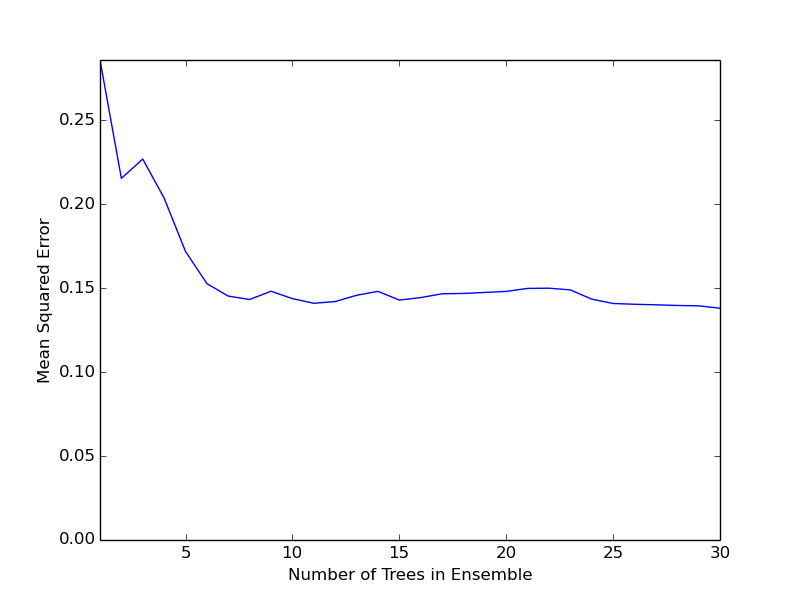
\includegraphics[width=0.5\textwidth]{mseEx2_ntm30td2na3}}
% 	\hfill
% 	\subfloat[mseEx2\_ntm30td5na3]{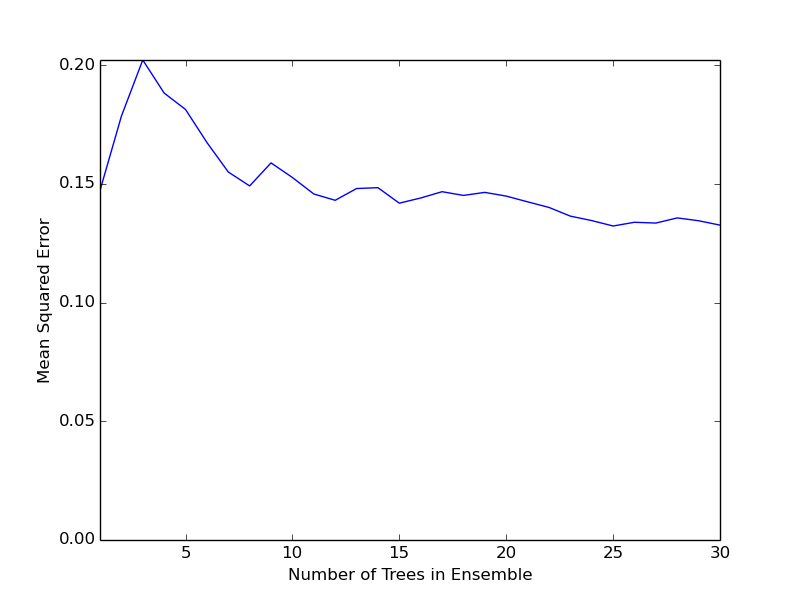
\includegraphics[width=0.5\textwidth]{mseEx2_ntm30td5na3}}
% \end{figure}
% \bigskip

Среди протестированных комбинаций минимум ошибки достигается
при размере ансамбля в 90 деревьев,
глубине дерева 12 и выборки в 4 признака для каждого дерева.

На самом деле данная реализация
не является в чистом виде random forest,
потому что в оригинальном алгоритме
в построение для каждого узла выбираются
своя выборка атрибутов.
Этот алгоритм правильнее было бы назвать
баггинг с случайным выбором признаков.
Данное несоответствие вызвано
невозможностью реализовать данную функциональность
через DecisionTreeRegressor.

\section{Пояснение}
Исходный код доступен по ссылке:
\href{https://github.com/SvichkarevAnatoly/Course-Python-Bioinformatics/tree/master/semester2/task10}
{github.com}

\end{document} % Конец документа
